%%%%%%%%%%%%%%%%%%%%%%%%%%%%%%%%%%%%%%%%%%%%%%%%%%%%%%%%%%%%%%%%%%% 
%                                                                 %
%                      Reeds gerealiseerd                         %
%                                                                 %
%%%%%%%%%%%%%%%%%%%%%%%%%%%%%%%%%%%%%%%%%%%%%%%%%%%%%%%%%%%%%%%%%%% 

\chapter{Reeds gerealiseerd}

Er zijn reeds een aantal experimenten uitgevoerd met de technieken die beschreven worden in de literatuur om voeling te krijgen met wat er wel en niet kan werken in situatie van dit onderzoek
en het beschikbare beeldmateriaal. De experimenten zijn onder te verdelen in 2 categorie\"{e}n die verder beschreven worden.

\section{Object detectie}
   In hoofdstuk~\ref{sec:trad_obj_det} is er beschreven hoe er op een traditionele manier pictogrammen herkent kunnen worden.
   Bij het zoeken naar de specifieke hue van de pictogrammen is gebleken dat het wel mogelijk is om dit als feature te gebruiken op het beschikbare beeldmateriaal, maar
   er is een te groot verschil in de belichting tussen de verschillende gangen waardoor de kleuren niet overeen komen en er moeilijk een juiste hue bepaald kan worden.
   Dit is ge\"{i}llustreerd in figuur~\ref{fig:kleurverschil}. Dit toont aan dat de hue van de pictogrammen geen absoluut uitsluitsel kan geven over de segmentatie, maar uitraard
   is het verschil in kleur in 1 beeld/omgeving nog steeds een feature die het pictogram onderscheid van de achtergrond.
   
   \begin{figure}[!htb]
      \centering
      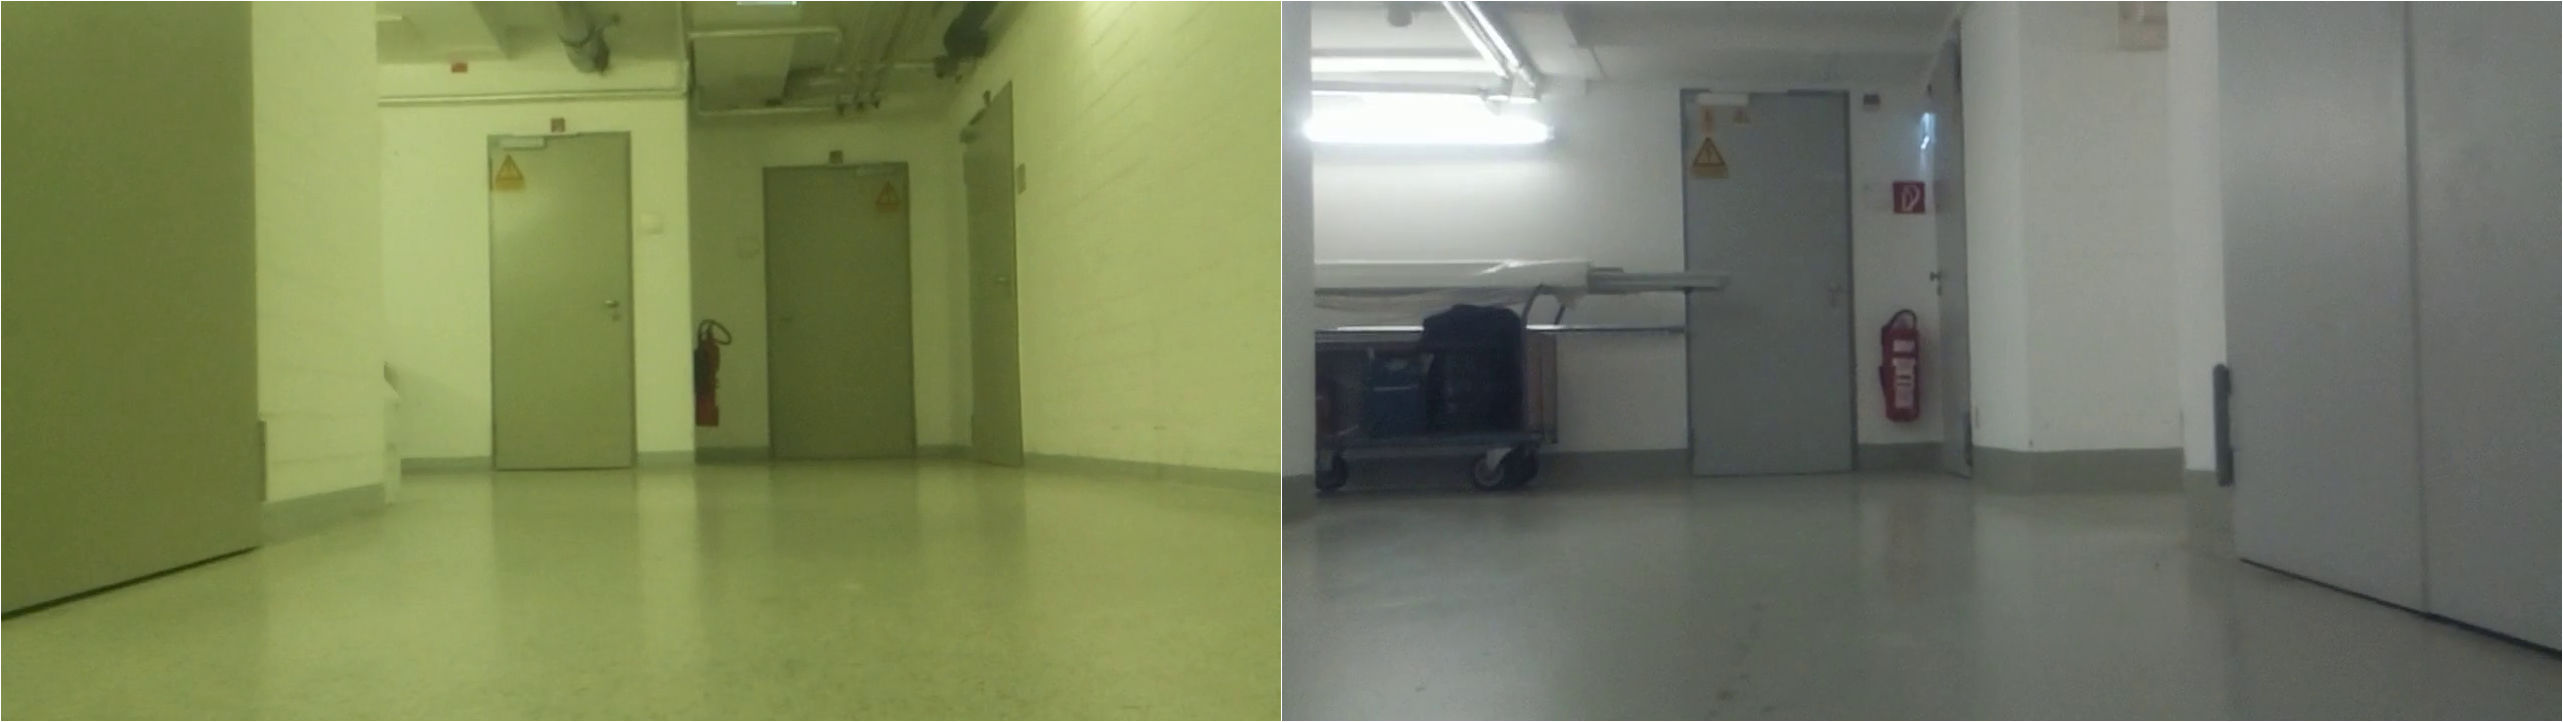
\includegraphics[width=0.75\linewidth]{kleurverschil.png}
      \caption{Kleurverschil tussen verschillende gangen}
      \label{fig:kleurverschil}
   \end{figure}

   Voor het identificeren van de pictogrammen is er geprobeerd om gebruik te maken van 'local feature matching' door middel van \gls{sift}. 
   Hierbij is gebleken dat door de lage resolutie van het beeldmateriaal er zo goed als geen features gedetecteerd kunnen worden zoals te zien in figuur~\ref{fig:sift_detect}.


   \begin{figure}[!htb]
      \centering
      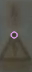
\includegraphics{sift_detectie.png}
      \caption{SIFT features op gedetecteerde contour.}
      \label{fig:sift_detect}
   \end{figure}


   In hoofdstuk~\ref{sec:yolo} is reeds beschreven hoe een \gls{cnn} gebruikt kan worden om objecten te detecteren. Hiervoor zijn we begonnen met annoteren van het beeldmateriaal.
   Voor het tekenen van bounding boxes is er gebruik gemaakt van de opencv tool CVAT\footnote{https://github.com/opencv/cvat}. Als proof of concept is er begonnen met 4 object klassen om te detecteren.

   \begin{itemize}
      \item Brandblusser
      \item Deurklink
      \item Pictogram
      \item Bordje
   \end{itemize}

   In elk frame van het beeldmateriaal zijn er voor deze klassen 'bounding boxes' getekend. De output van de CVAT tool is een XML-bestand met voor elke afbeelding de co\"{o}rdinaten van de objecten.
   Een voorbeeld output voor 1 enkele afbeelding is te zien in listing~\ref{lst:cvat_xml}.

   \lstset{language=XML, caption={Voorbeeld CVAT output}, label={lst:cvat_xml}}
   \begin{lstlisting}
<image id="24" name="hospital_corridors_4Hz-025.png" width="1280" height="720">
   <box label="door_handle" xtl="863.66" ytl="237.20" xbr="881.28" ybr="248.22"/>
   <box label="sign" xtl="584.02" ytl="254.12" xbr="608.24" ybr="265.28"/>
   <box label="door_handle" xtl="435.83" ytl="321.53" xbr="448.33" ybr="329.06"/>
   <box label="sign" xtl="590.76" ytl="298.63" xbr="604.02" ybr="307.70"/>
</image>     
   \end{lstlisting}

   De trainingsdata die aan het \gls{yolo} netwerk geleverd moet worden is een volledig ander formaat dan het verkregen XML bestand, daarom is er een conversiescript geschreven om dit om te zetten naar het \gls{yolo} formaat.
   Het conversiescript bevind zich in bijlage~\ref{bij:convert}. 
   Het formaat dat \gls{yolo} verwacht is per input afbeelding een .txt bestand met daarin per lijn een bounding box. Het \gls{yolo} formaat is beschreven in~\ref{eq:yolo} waarbij $<x>$ en $<y>$ het centerpunt van een bounding box zijn.

   \begin{equation} \label{eq:yolo}
      <x> <y> <width> <height> 
   \end{equation}

   In figuur~\ref{fig:yolo_1} en~\ref{fig:yolo_2} zijn 2 resultaten te zien van de \gls{yolo} detector op de dataset.

   \begin{figure}[H]
      \centering
      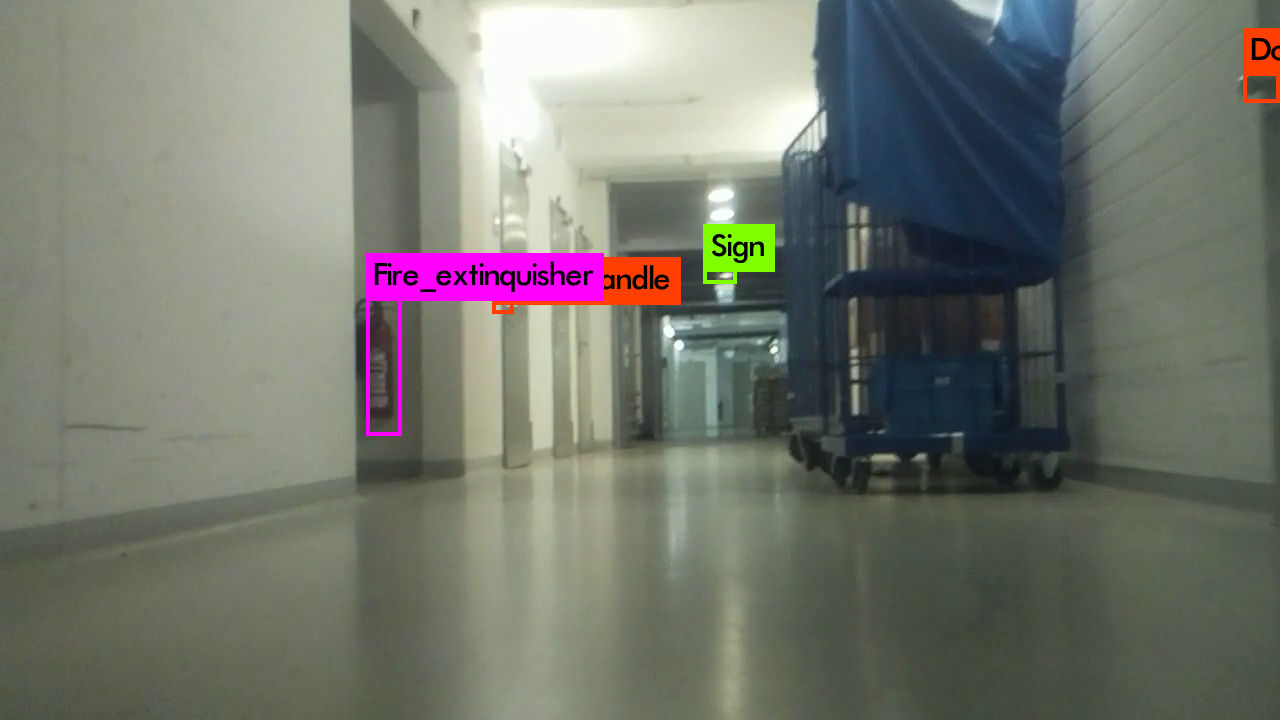
\includegraphics[width=0.75\linewidth]{yolo_detectie1.jpg}
      \caption{Resultaat 1 YOLO detector.}
      \label{fig:yolo_1}
   \end{figure}

   \begin{figure}[!htb]
      \centering
      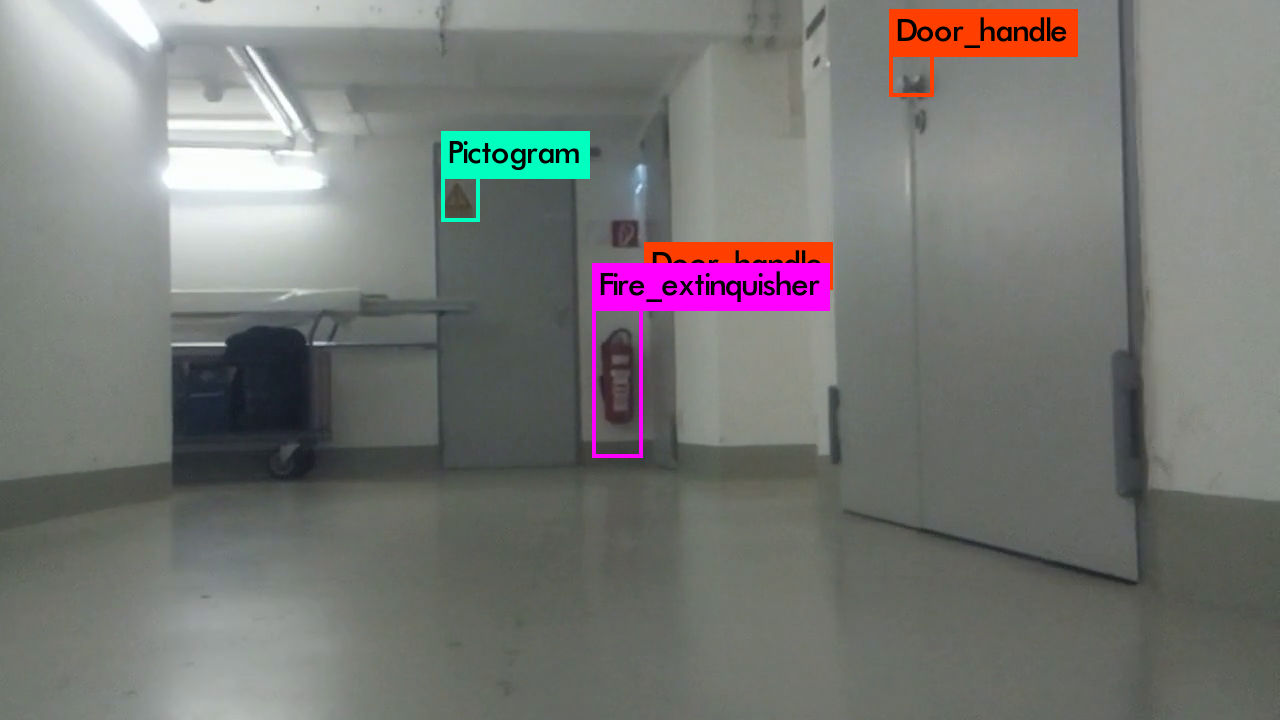
\includegraphics[width=0.75\linewidth]{yolo_detectie2.jpg}
      \caption{Resultaat 2 YOLO detector.}
      \label{fig:yolo_2}
   \end{figure}

\newpage
\section{Image segmentation}

   Zoals reeds voorgesteld in hoofdstuk~\ref{sec:image_segmentation} kan voor het segmenteren van de gangen gebruik gemaakt worden van het SegNet~\cite{Badrinarayanan} segmentatie netwerk.
   Na enkele uren proberen is het niet gelukt om SegNet werkend te krijgen. Dit zal in de toekomst hernomen worden.

   In plaats daarvan is er een ander segmentatie netwerk gevonden gebaseerd op ResNet dat reeds getraind werd op een dataset met indoor scenes en gangen.
   In figuur~\ref{fig:resnet_seg} is het resultaat te zien van het netwerk zonder een hertraining.

   
   \begin{figure}[!htb]
      \centering
      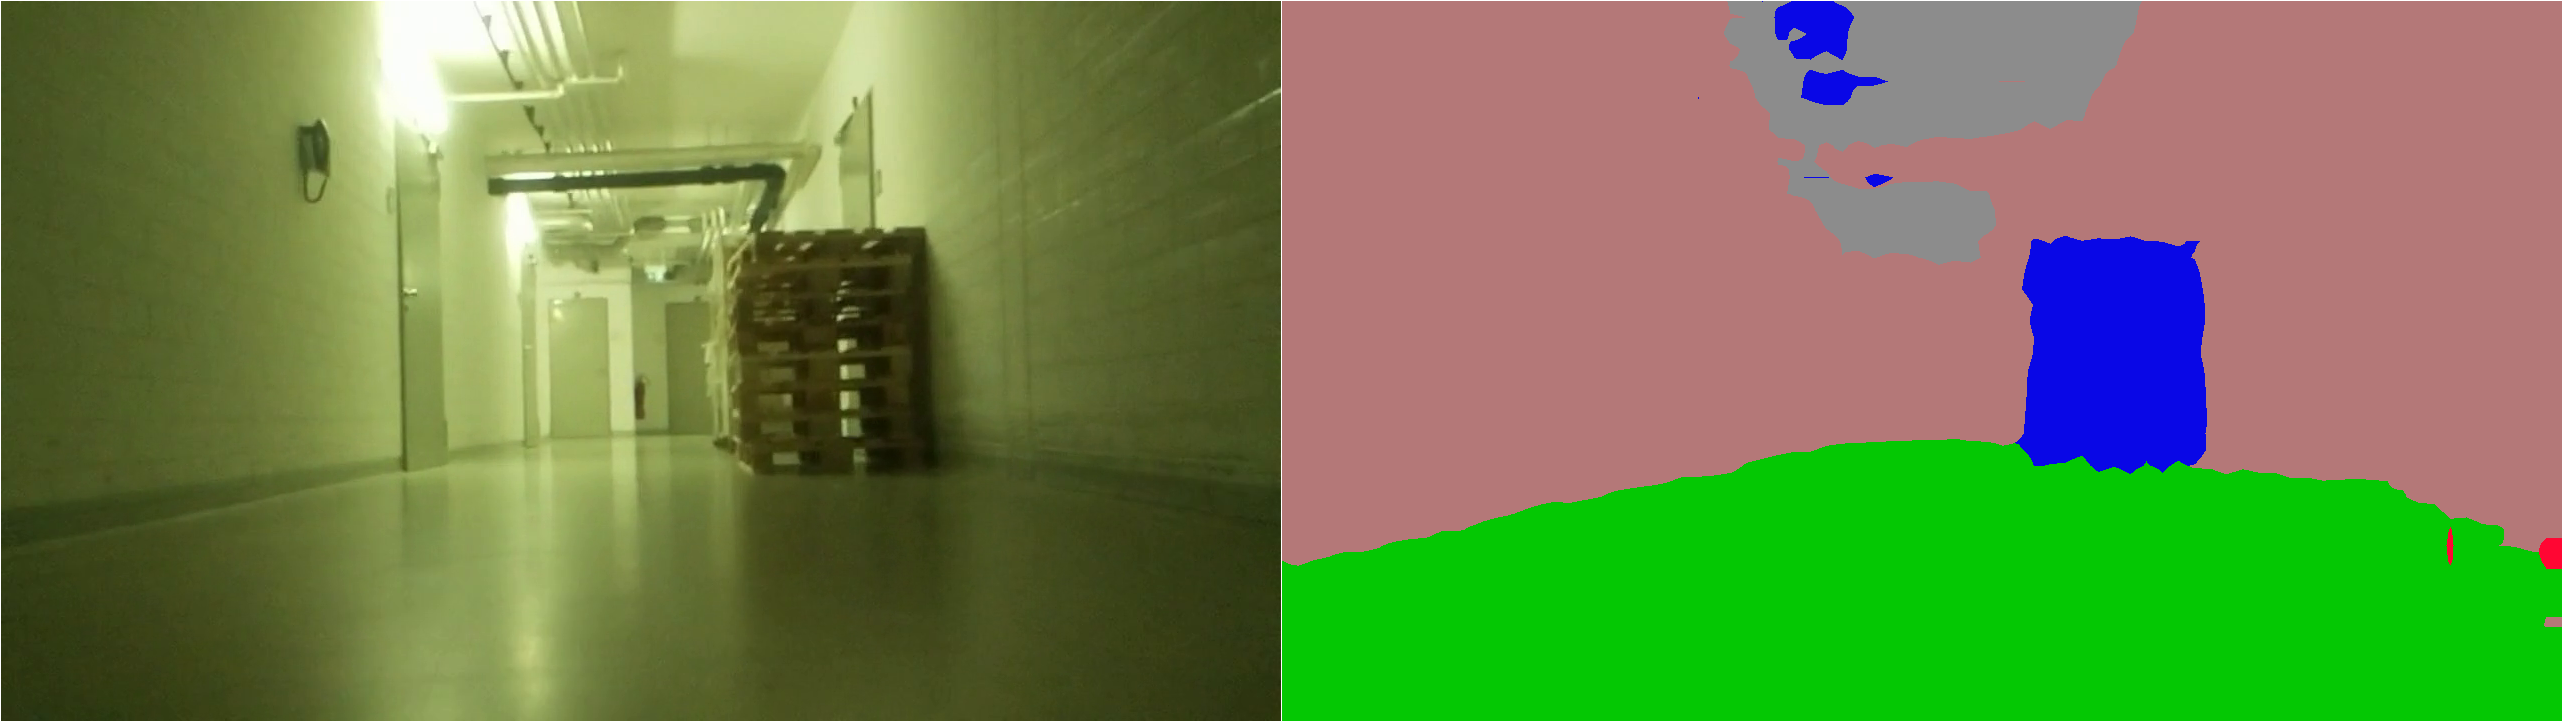
\includegraphics[width=0.75\linewidth]{resnet_segmentatie.png}
      \caption{Resultaat van ResNet segmentatie netwerk.}
      \label{fig:resnet_seg}
   \end{figure}

   In de toekomst zal er vergeleken welk van de 2 netwerken het beste resultaat geeft, en zal er een hertraining gebeuren op basis van het beeldmateriaal om te proberen om ook deuren te segmenteren.